\chapter{Representations of sound actions}

`Why don't you try to map the perceptual features instead?' one of my Ph.D. colleagues asked as I pondered how to control a sound engine with an electromagnetic motion tracking system. Until then, I had mainly thought about mapping as a technical procedure. You acquire some control signals that are processed a little before routing them to a feature in the sound engine. I had not thought about the possibility of creating higher-level or multi-layer mappings. It occurred to me that it is also possible to perform more advanced feature extraction on the control side and think about perceptual features on the sound engine side. Indeed, it is easy to forget that music theory is at a much higher level of abstraction than sound theory when you are stuck with reading in raw sensor signals and figuring out ways to pass all the data forward in a processing chain. From then on, I turned my attention towards `perceptual mapping.' This chapter will look at my proposed Gesture Description Interchange Format (GDIF) and why it failed. But first, we will take a look at traditional musical notation and the commercial standards MIDI and MPE. After all, they, too, are formal representations of musical information based on perceptual features.


\section{Coding actions in musical scores}

It may not be evident to everyone, but traditional musical scores are a form of action notation. A \emph{note} in a musical score is a description of how a \emph{tone} is going to be played. Figure~\ref{fig:score} shows an elementary score, containing only a few notes. The beauty of musical notation is that it manages to carry a lot of information in an incredibly compact visual representation. For example, the vertical position of a note in the score tells which pitch to play. This assumes that one knows the \emph{clef}, which serves as a reference point of the score. The score in Figure~\ref{fig:score} is written in `treble clef.' This means that the second line from the bottom represents the tone G. In addition, it is necessary to check whether there are any signs at the beginning of the system that indicates the  \emph{key} of the tune (here, D major or B minor). In the example, there are two \musSharp\ written at the beginning of the score, which means that all the F and C notes should be played sharp, that is, as F\musSharp\ and C\musSharp, respectively. This is unless there is a \musNatural\ sign in front of a note, which would remove one of the global signs. In addition, there could also be extra \musSharp\ or \musFlat\ signs for single notes. It should be said that the whole system is based on a twelve-tone equal temperament scale, so the steps between notes in the score are unequal. There are whole steps between some notes (C--D, D--E, F--G, and A--B) and half steps between others (E--F and B--C).

\begin{figure}[tp]
	\centerline{
	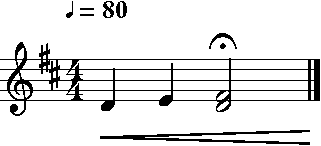
\includegraphics[width=0.4\columnwidth]{figures/31-simple-score-crop.pdf}
	\caption{A musical score contains a lot of information in a compact visual representation.}
	\label{fig:score}
}
\end{figure}

There are also tuning differences to take into account. In the example in Figure~\ref{fig:score}, the first note will be interpreted as the tone D. However, that D will not necessarily sound the same when played on different instruments. If played on the piano, the tone will most likely have a frequency of around 293~Hz. If you play the same D on a regular trumpet (tuned in Bb), it will sound like the C on the piano, while a D played on an alto saxophone (tuned in Eb) will sound like an F. So the instrument matters a great deal when turning notes into tones.

There are also micro-tuning differences between instruments. When I mentioned that a D played on the piano results in a tone with a fundamental frequency of  293~Hz, this was based on the assumption that the piano is tuned in a performance pitch of 440~Hz. The performance pitch is usually defined by the frequency of the note A above middle C. While 440~Hz is a standard tuning today, \citet{haynes_history_2002} has documented that the `A' has had many different pitches throughout history. And also today different ensembles explore other tunings.

For musicians playing alone, the exact tuning does not matter. The most important is that the instrument is tuned relative to itself. So whether the instrument is tuned in A=430~Hz or A=450~HZ, does not matter for people without perfect pitch. That said, many musicians use auto-tuners these days, and they are typically based on a frequency of A=440~Hz. So are most commercial electro-acoustic instruments, such as digital pianos. Various digital audio workstations may also be set up to work best with a standard tuning of A=440~Hz. Thus, new technologies have lead to a standardized tuning practice.

What is fascinating is that musical scores are both absolute and relative at the same time. The score attempts to specify an absolute ratio between notes, but these ratios are relative at many levels. The performer needs to `calculate' the right note based on knowledge about music theory. In addition, a score also contains both absolute and relative temporal information. The position of notes from left to the right tells the performer about the \emph{order} of tones to be played. However, as opposed to the even distribution of points on the x-axis in data plots, a musical score does not base its timing on the notes' exact position on the page. It is a note's value---such as \musWhole\ \musHalf\ \musQuarter\ \musEighth\ \musWholeDotted\ \musHalfDotted\ \musQuarterDotted---that tells how long it should be played. These relative durations can be made even more relative by using a fermata sign.
%todo: should add a fermata sign here
Scores also often have a tempo indication. This could be a relative representation, such as `Andante,' which would indicate a tempo in the region of around 70-100 beats per minute on a metronome. There could also be a fixed number (\musQuarter\ = 80) prescribing the intended beats per minute. However, how precisely such a number is interpreted is up to the performer.

In addition to frequency and time information, a score may contain loudness information, usually specified in relative terms. It can either be through a textual description (\emph{ppp}---\emph{FFF}) or a crescendo line, as in Figure~\ref{fig:score}. Finally, a score may contain `absolute' information about timbre by specifying an instrument. Additional `relative' timbre information can be added through descriptions of playing techniques. For example, in violin scores, the performer would play with a bow if nothing else is specified. But if \emph{pizz.} is written, the performer would play with the fingers instead.

Given the large `gap' from note to tone, much interpretation is left to the performer. I still remember one of my first composition classes, in which we were given the task of writing a short cello piece. I had made my score in notation software and had listened to the piece using the simple MIDI playback device available in the software. This had rendered the melody sufficiently well to understand how it could sound. However, hearing the piece performed by a live musician, with the beautiful cello sound right in front of me, was mind-blowing. It was a compelling manifestation of the difference between notes and tones.

Musical scores have developed over many centuries to become a powerful and flexible tool for composers and musicians \citep{grier_musical_2021}. Many composers have used scores as their primary method to communicate musical intentions in the Western art music tradition. Music researchers have also embraced scores as a method to study musical structures and composers' intentions.
This does not only include music that was notated from the start. It has also been a tradition of transcribing sounding music into written scores for later analysis, such as jazz improvisations or folk tunes. However, one should always be careful about simplifying and interpreting such `translations' from one representation to another.


\section{Chord notation}

The note-based musical scores mentioned above are just one of several ways that musical information can be coded. Another commonly used score type is that of chord notation. Such notation is typically found in books of popular songs or jazz tunes and is even more `action-based' than traditional music notation. Chord notation is based on providing only information about the chords to be played. For example, a standard jazz chord sequence can be written as Dm7, G7, C. Those familiar with this type of notation know that Dm7 includes the tones D-F-A-C, G7 consists of the tones G-B-D-F, and C has C-E-G. If this were a jazz tune, many would probably also think that the C is a short-form of writing Cmaj7, including the major 7 in the chord (C-E-G-B). Someone familiar with jazz theory would immediately be able to improvise a melody if they were given a sequence like Dm7, G7, C. Thus, such a sequence is an even more compact way of representing musical information than a note-based score. It also requires even more knowledge about music theory and the particular genre in question.

While it is common to write out both the note name (D) and the chord structure (m7), the representations could be even more compact. In functional harmonic analysis, it is common to write IIm7, which would be a relative pitch representation. In the example above, II would represent the second note (D) of the scale of the fundamental note (C). In genres where there is a clear understanding of how the harmonic structures relate to each other, it may be sufficient to write the above example as II, V, I. This would be sufficient to understand which chords and tones to play. Writing notes with such a functional representation also makes it easier to transpose a tune to a different key. For example, if I would like to play the tune in G major instead of C, the II, V, I sequence would be played as Am7, D7, G. Such translations between different representational systems is standard procedure for many musicians.

Some people find it challenging to remember which notes to play from chord notation. For that reason, some guitar books contain fretboard diagrams, such as shown in Figure~\ref{fig:guitar-chords}. These are visual representations of the guitar neck, indicating open strings and the frets that it is necessary to hold to get the right chord. How to play them, however, is up to the performer. One can strum the guitar strings, thereby playing all tones at (almost) the same time. Or one can play the bass tone followed by the other tones. Chord notation contains no timing information beyond indicating when one should change from one chord to another. I find it interesting that various types of music notation, whether note-based or chord-based, are predominantly based on representing actions. In guitar chord notation, it even contains a simplified representation of a part of the instrument.

\begin{figure}[tp]
	\centerline{
	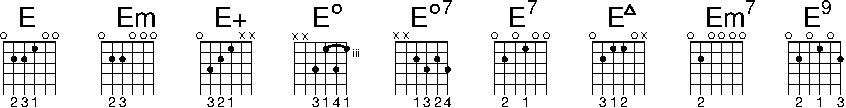
\includegraphics[width=1\columnwidth]{figures/32-fretboards.pdf}
	\caption{Chord notation (top) with corresponding guitar fretboard diagrams.}
	\label{fig:guitar-chords}
}
\end{figure}

\citet{magnusson_sonic_2019} discusses how musical scores have developed over the centuries and how this has shaped musical creation and thinking. This includes the traditional note- and chord-based scores mentioned above and various types of computer code and other representations of musical tones and ideas. The experimentation with extended techniques on acoustic instruments leads to the continuous expansion of the symbols used in scores, although many of these are not standardized. Also, compositional experimentation leads to new types of scores. While traditional, linear scores still prevail, examples of circular or fragmented scores allow for more flexible performance. The addition of new electro-acoustic instruments continues to push for new notation forms, both on paper and on-screen. Some graphical music programming languages (such as PureData and Max) may contain score information in the graphical user interface itself. Other languages, such as CSound upholds a clear separation between sound (`orchestra') and structure (`score') \citep{boulanger_csound_2000}. Despite these differences in representation---spanning from traditional to experimental score types---there is a need to represent information about musical tones and musical structure. In computers, this is most commonly done with the MIDI format.


\section{The Musical Instruments Digital Interface (MIDI)}\label{sect:midi}

When electro-acoustic instruments, particularly various types of keyboard-based synthesizers, became popular in the 1970s and early 1980s, it became clear that there was a need to standardize the communication between devices. This led to the development of the \emph{Musical Instruments Digital Interface} (MIDI) format, which the MIDI Association proposed in 1983, and has been the de facto instrument communication standard ever since \citep{jungleib_general_1996}. The MIDI standard provides a simple way of connecting controllers to sound engines by defining the physical cables used to connect devices and the protocol used for the communication. The MIDI standard does not specify mappings between controller and sound, but the General MIDI (GM) specification, and Roland's General Sound (GS) extension, define specific timbre sets. This makes it possible to play a MIDI file on any GM compliant system and get a more or less similar rendition of the music.

MIDI is one of the most successful and oldest standards in the computer industry \citep{rothstein_midi_1992}, and one which is still going strong. That is the case even though it was met with criticism already from the start. Both \citet{loy_musicians_1985} and \citet{moore_dysfunctions_1988} criticized MIDI for its low resolution, high latency, number-based messaging structure, and serial nature. While each of these weaknesses may not be that problematic in itself, the combination often led to challenges, particularly in large setups. Several of these problems have later been solved or marginalized in various ways. For example, MIDI signals were traditionally passed over 5-Pin DIN MIDI cables, but it is now more commonly transmitted through USB cables. The growing processing speed has also helped in reducing latency problems. So for many use cases, MIDI is good enough for the task at hand.

In the context of this book, my main interest in MIDI is its conceptual design, particularly the use of `notes' as the central organizing unit. MIDI communication is built around sending \emph{note-on} and \emph{note-off} messages using a twelve-tone equal temperament system to denote the pitch values. This fits well with the traditional, Western music notation systems described above. It also works well with the discrete nature of keyboard-style controllers, modeled after the piano's sound-producing actions. In fact, for such impulsive actions and sounds, MIDI provides a highly efficient representation. However, such an impulsive-based representation is challenging for continuous controllers and sustained sound engine types. For example, representing a continuous pitch slide with MIDI requires the use of a series of note-on, note-off and pitch-bend messages. Working with micro-intervals is equally problematic, as one would need to send tempered pitch messages together with a pitch-bend message denoting the `detuning' of each note.

The MIDI standard encourages impulsive-like sound control. One can, therefore, only wonder whether the MIDI standard itself is a reason for the proliferation of keyboard-based and `knobs-and-sliders'-type controllers.
Since only the tone's attack can be controlled directly---with information about its pitch and the initial velocity---the rest of the tone has to be controlled programmatically. This can be done through the use of \emph{envelopes}, such as the attack-decay-sustain-release (ADSR) envelope (Figure~\ref{fig:electroacoustic4}). Many synthesizers allow modifying the amplitude and duration of each part of such an envelope using separate controllers. This can sometimes be done during a performance, although it would mean that the performer moves one or two hands away from the keys. It is more common to adjust such settings between songs.

\begin{figure}[tbp]
	\centerline{
		  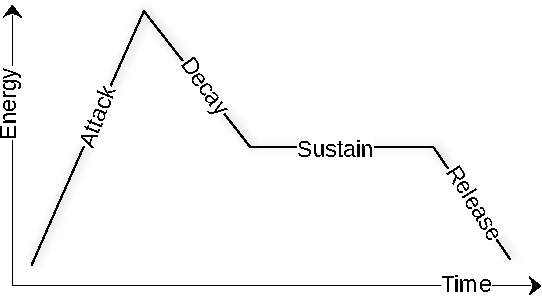
\includegraphics[width=0.7\textwidth]{figures/33-adsr-crop.pdf}
			\caption{A sketch of an ADSR envelope, which is commonly used to shape the tone's amplitude in electro-acoustic instruments.}
			\label{fig:electroacoustic4}
}
\end{figure}

\emph{Low-frequency oscillators} (LFOs) are another group of temporal control messages that are common to use in synthesizers. These are time functions designed to continuously change the shape of sounds and their timbral/textural features. An LFO can be anything from a low-frequency sine-tone to complex multi-frequency signals. In some cases, they may also include rhythmic, melodic, or harmonic elements. As we will discuss later, such processes are part of the change from `sound-makers' to `music-makers.' For the performer, such long semi-automatic processes may feel like the instrument plays `itself.' In some cases, the system may even be designed so that the performer knows when to release the key. \citet[p.77]{lossius_sound_2007} reflects on how such procedural processes may lead to the instrument controlling the performer rather than the other way around. Most synthesizers allow for programming both envelopes and LFOs in various ways, and parts of the creative process may be spent on making \emph{presets} for a performance. In some cases, entire pieces can be composed by solely setting up synthesizer presets. Synthesizer manufacturers have for a long time understood the importance of providing high-quality presets with their devices. Users appreciate products that have a varied set of presets available. There is even a market for selling and buying presets that extend synthesizers' possibilities.


\section{MIDI Polyphonic Expression}\label{sec:mpe}

After many years of discussion about how to extend the MDI standard, the MIDI Polyphonic Expression (MPE) extension was finally agreed on in 2018 \citep{the_midi_association_midi_2018} followed by the MIDI 2.0 specification two years later \citep{the_midi_association_midi_2000}. These extensions came out of the need for interoperability of new keyboard-based instruments with continuous control (which we will look more at in Chapter~\ref{sec:mpe-instruments}). The new standards are implemented conservatively, meaning that they are backward compatible with the original MIDI specification.

The MPE standard is implemented using MIDI channel 1 for sending global messages. The remaining channels transmit notes and `expressive' data, including note-on velocity, pitch bend, channel pressure (aftertouch), brightness, and note-off velocity, on a note-per-channel basis. This makes it possible to send richer messages than what is possible with traditional MIDI streams while still staying within the MIDI ecosystem. A similar approach is taken in MIDI 2.0, but here with a broader implementation based around a MIDI Capability Inquiry (MIDI-CI) system \citep{the_midi_association_common_2020}.

MPE and MIDI 2.0 solve some of the problems with the original MIDI standard, but not all. The standards are still focused on keyboard-based control and the concept of note-on and note-off messaging. Even though it now supports continuous control, the MIDI standard is still not a generic solution for object-based sonic interaction.


\section{Open Sound Control}

It is easy to spot problems with the MIDI standard, but it is challenging to develop alternative solutions. Throughout the years, there have been several failed attempts. The most successful alternative is \emph{Open Sound Control} (OSC), which was proposed by a team of researchers at the Center for New Music and Audio Technologies (CNMAT) at the University of California, Berkeley in the 1990s \citep{wright_open_1997}. Over the years, OSC has become the de-facto communication standard in the music technology research community \citep{jensenius_open_2017}, and it is also used in some commercial products.

OSC was designed as a general communication protocol and can be used over many different cable types, including Ethernet, USB, or even MIDI cables. It adopts a URL-style messaging format, such as:

\begin{verbatim}
	/voices/3/freq 400
\end{verbatim}

\noindent
which refers to sending the message $400$ to the module $freq$ inside a node $3$ that is a child of the top-level node $voices$. As opposed to MIDI's serial messaging nature, OSC supports pattern matching. This means that it is possible to send messages like:

\begin{verbatim}
	/voices/*/freq 400
\end{verbatim}

\noindent
to control the frequencies of several voice modules in parallel.
OSC's text-based labeling structure allows for sending meaningful messages between devices. This makes the protocol more human-friendly than the number-based approach used in MIDI messages. Still, OSC has been criticized for being too light-weight \citep{dannenberg_o2:_2016}. It relies on IP addresses and port numbers without handling human-friendly device names.

As the name implies, OSC is an open standard where few limitations are forced upon the user. This openness is both a strength and a limitation.
MIDI is based on the `note' as a core sonic/musical entity, and any MIDI-compliant interface could be connected to any sound engine. OSC allows the user to create any message. That may be liberating at first, but the result is that OSC-based devices and software cannot communicate directly without first setting up specific mappings between them. Already from the start, it was suggested that working towards standard guidelines and creating uniform namespaces was important \citep{wright_managing_2001}. However, except for a few examples---of which the TUIO standard for table-based tangible user interfaces is the most prominent \citep{kaltenbrunner_tuio_2005}---such standardization has not happened. That may be one reason that OSC has gained  most traction in the research community, in which people are more inclined to develop namespaces themselves.


\section{Gesture Description Interchange Format}\label{sec:gdif}

My interest in developing a higher-level mapping system for control interfaces and sound engines led to the proposal of the \emph{Gesture Description Interchange Format} (GDIF) \citep{jensenius_towards_2006}. This was an ambitious project, aiming to create more human-friendly mappings from action to sound. The dream was to have a system that would allow for mapping between multiple data streams, ranging from low-level sensor data to higher-level control features, such as sketched in Figure~\ref{fig:gdif-streams}.

\begin{figure}[tbp]
 			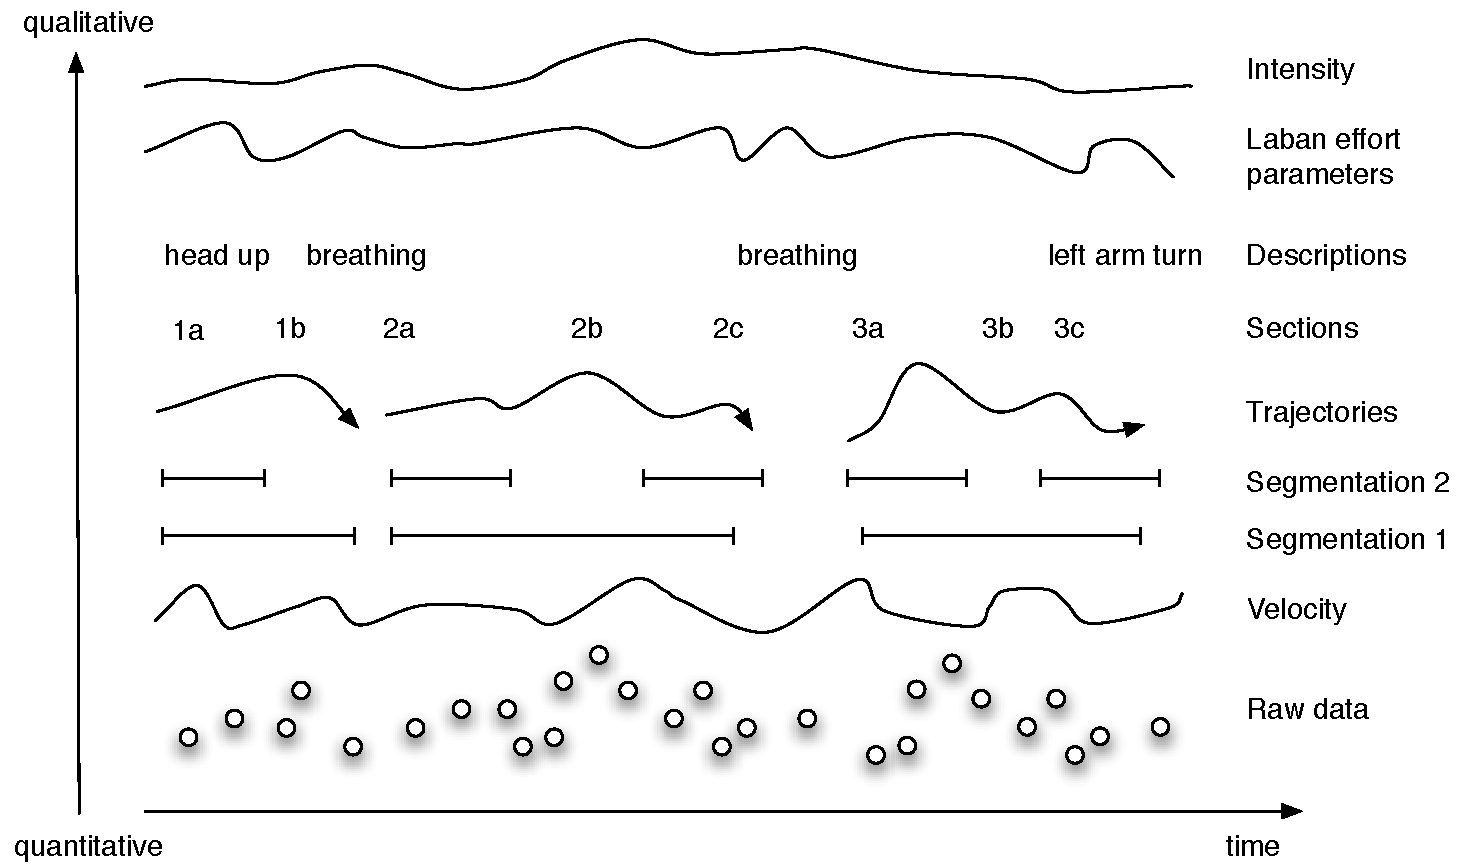
\includegraphics[width=1\columnwidth]{figures/34-gdif-streams.pdf}
 			\caption{Sketch of different levels of data that could be streamed with GDIF.}
            \label{fig:gdif-streams}
\end{figure}

Inspired by the ESCHER system of \citet{wanderley_performer-instrument_2001}, GDIF aimed at using \emph{intermediary} mapping layers. Instead of mapping directly from technical action parameters to technical sound parameters, the user would map between perceptually meaningful parameters (Figure~\ref{fig:gdif-namespace}).
For example, mapping the position coordinates of a joystick onto the center frequency and gain of a filter may seem logical to people with music technological experience. However, such a technical mapping would probably not be intuitive for most others. A more ecological approach would be to create mappings based on the action used (`move the right hand to the right') and the perceptual quality of the sound (`change the brightness and loudness of the sound').

\begin{figure}[tbp]
 			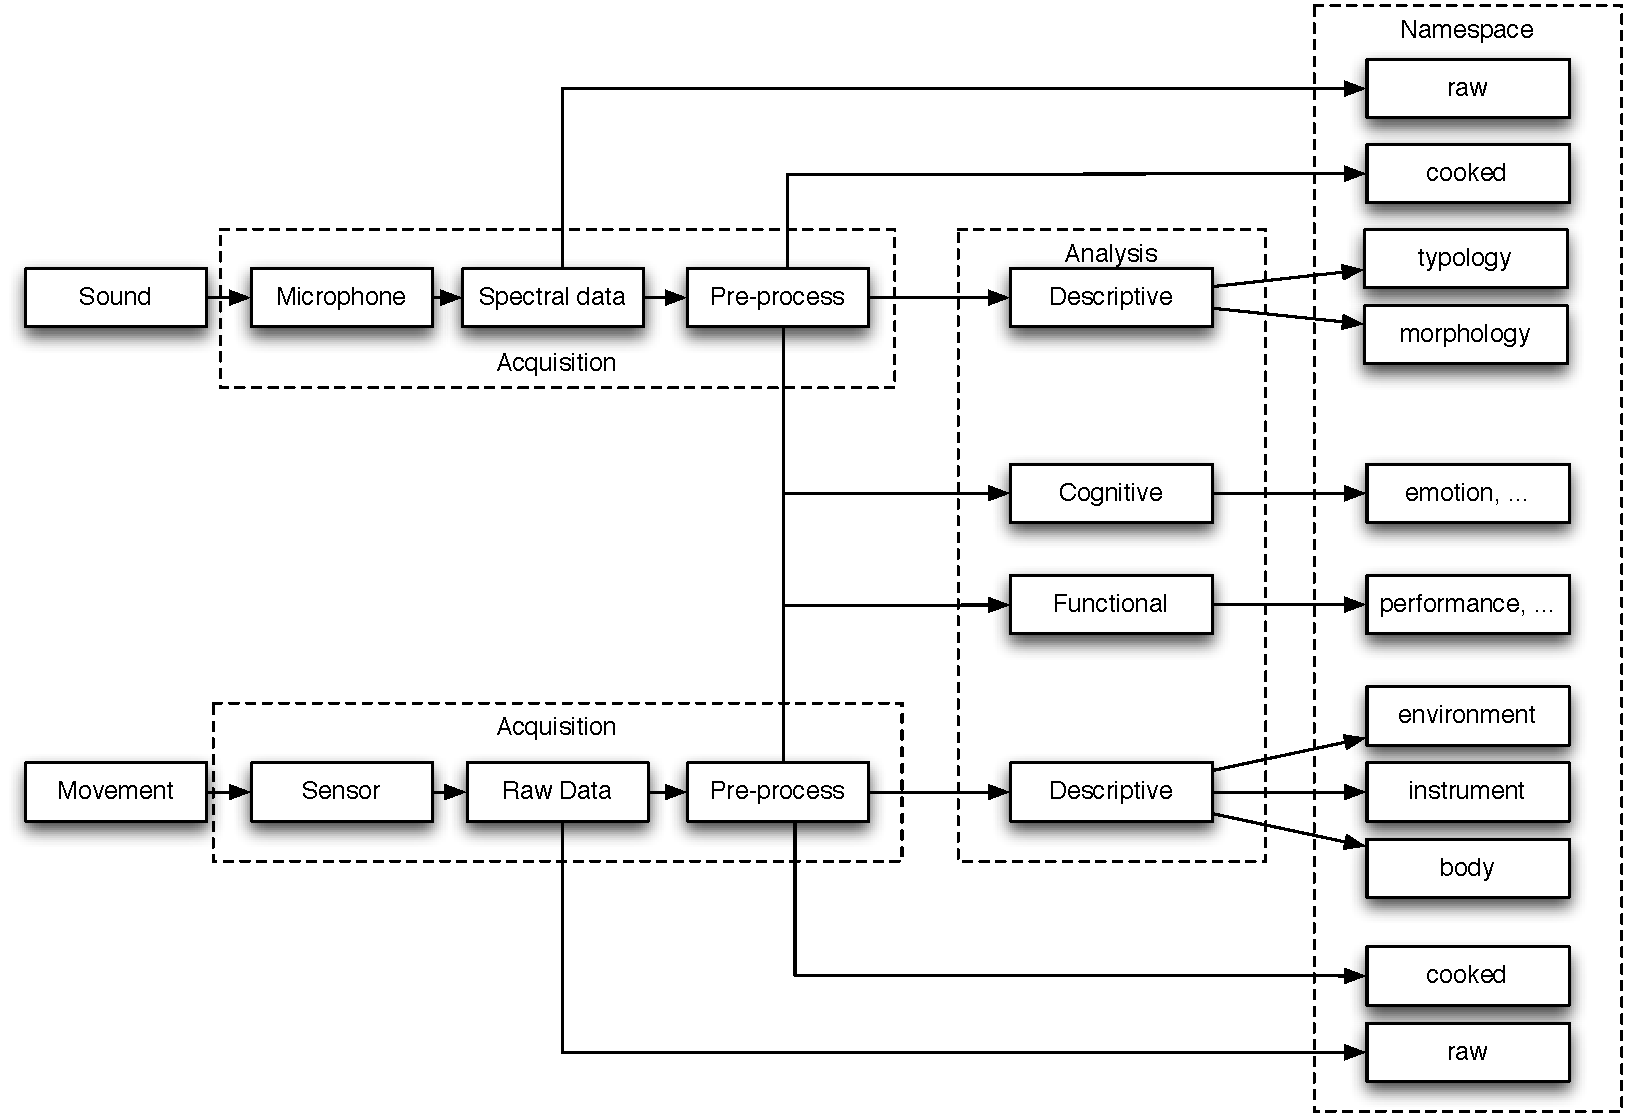
\includegraphics[width=1\columnwidth]{figures/35-gdif-namespace.pdf}
 			\caption{Sketch of the multilayered namespace proposed for GDIF.}
            \label{fig:gdif-namespace}
\end{figure}

The idea was to base mappings on meaningful parameters and allow for interchanging controllers and sound engines. So the perceptual mappings would remain while the technical mappings would change. For example, if I want to use a lateral hand action to control a sound, it should not matter what type of motion capture system I use to track information about the action. A camera-based or sensor-based system will have different numerical representations of the motion in question. However, as long as these are first mapped into a meaningful motion-based mapping layer, this layer can be used for mapping onto perceptually meaningful sound features. On the sound side, one could imagine a similar type of intermediate mapping layer between perceptually meaningful sound features and the technical features of the particular sound engine.

I still think that the conceptual idea of GDIF is good, but it is challenging to implement. I created some mapping examples that worked well. However, scaling up to a general solution showed how challenging it is to handle all the nuances and complexities of musical instruments. It would certainly be possible to develop coarse generic mappings, but I doubt that the dream of creating a genuinely generic mapping system could ever work. If so, machine-learning-based approaches have proven to be more successful in achieving such a goal \citep{fiebrink_wekinator_2011}. Then the user can choose to train the system based on perceptually meaningful actions and sounds. Given the `black box'-nature of such models, the user would not get a meaningful representation of the mapping. However, that may not necessarily be a problem if the mapping works as expected.

I have used machine learning in some of my instruments, but many of the instruments I will present in later chapters are based on basic technical mappings. After working on more sophisticated mapping systems for some years, I discovered that creating coupled mappings between a few technical parameters can work quite well. This also gives some `resistance' to an instrument that may spark creativity. However, from a conceptual perspective, I still think it is an interesting exercise to reflect on the possibility of creating perceptually based mappings.
